\label{chap2}

This chapter describes the derivation of a dynamic model of the soft robotic manipulator. First, the soft robotic system considered in this work is detailed. Then, the configuration space of the soft robot is described. Once this configuration space is determined, the forward kinematics at position and velocity level are derived. These forward kinematics are useful for deriving the dynamic model of the soft robot. Additionally, a model is provided that is utilized to describe the pump dynamics. Lastly, the state-space representation of the combined system dynamics is presented, which combines the dynamics of the soft robot and pump dynamics.


%%%%%%%%%%%%%%%%%%%%%%%%%%%%
%%%%%%%%%%%%%%%%%%%%%%%%%%%%f

\section{Soft robot manipulator description}

The soft robot manipulator studied in this work is composed of a visco-elastic polymer using selective laser sintering technology. This manufacturing method is well suited to print hollow compartments, that allow for inflation. The elastomer has a low Young's modulus and can sustain large strains. These characteristics allow inducing large deformations with relatively low pressures. The geometry of the soft robot is best described by two bellows placed in parallel. Over the vertical axis, the bellows are connected, creating the centre line of the robot. The bellows are connected by flanges at the top and bottom. The bellows can be inflated individually via air inlets created in the flange at one end of the robot. The other end is closed, allowing to pressurize the bellows. Since each bellow can be inflated independently, the entire robot can increase its length and change orientation. Pressurizing both bellows equally will result in a near pure elongation of the soft robot. Creating a pressure difference will cause the soft robot to bend. The following assumption is made concerning the robot's task-space:

\begin{theorem}
Strains in the soft robot imposed by pneumatic actuation change the soft robot's length and orientation. Strains causing out of plane motion are deemed negligibly small, and can not be actively regulated. The manipulator's task-space restricts itself to a single plane, reducing it to a 2-dimensional problem.
\end{theorem}

This assumption allows describing the configuration of the soft robot in a two-dimensional Cartesian plane. Since the soft robot has no clear end-effector in the form of a gripper, a point on the body is assigned to be the end-effector. This point is situated at the geometric midst of the closed flange, see Figure \ref{fig2:setup}. The flange with the air inlets is fixed, here its geometric midst is defined as the origin. Altering the bellow pressure can therefore change the soft robot's end-effector position. Based on the above assumptions a kinematic model of the soft robot is developed using the Cosserat beam model. 



\begin{figure}[H]
\begin{minipage}{.5\textwidth}
  \centering
  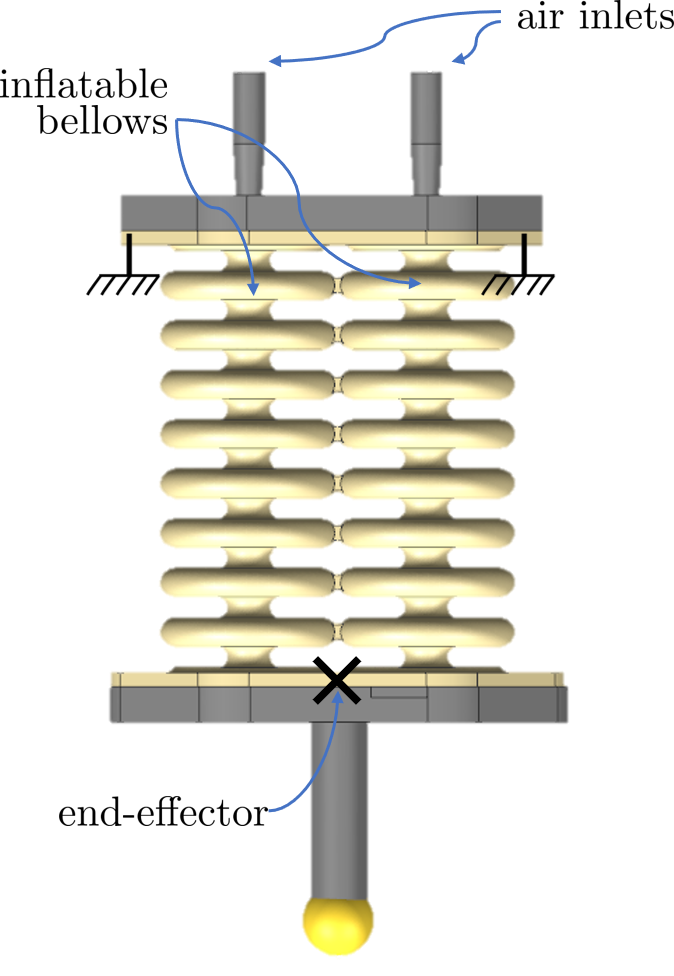
\includegraphics[width =0.8\linewidth]{Figures/Chapter2/setup.png}
  \caption{Schematic drawing of the soft robot manipulator setup, denoting its fixation points and end-effector location.}
  \label{fig2:setup}
\end{minipage}
\begin{minipage}{.5\textwidth}
  \centering
    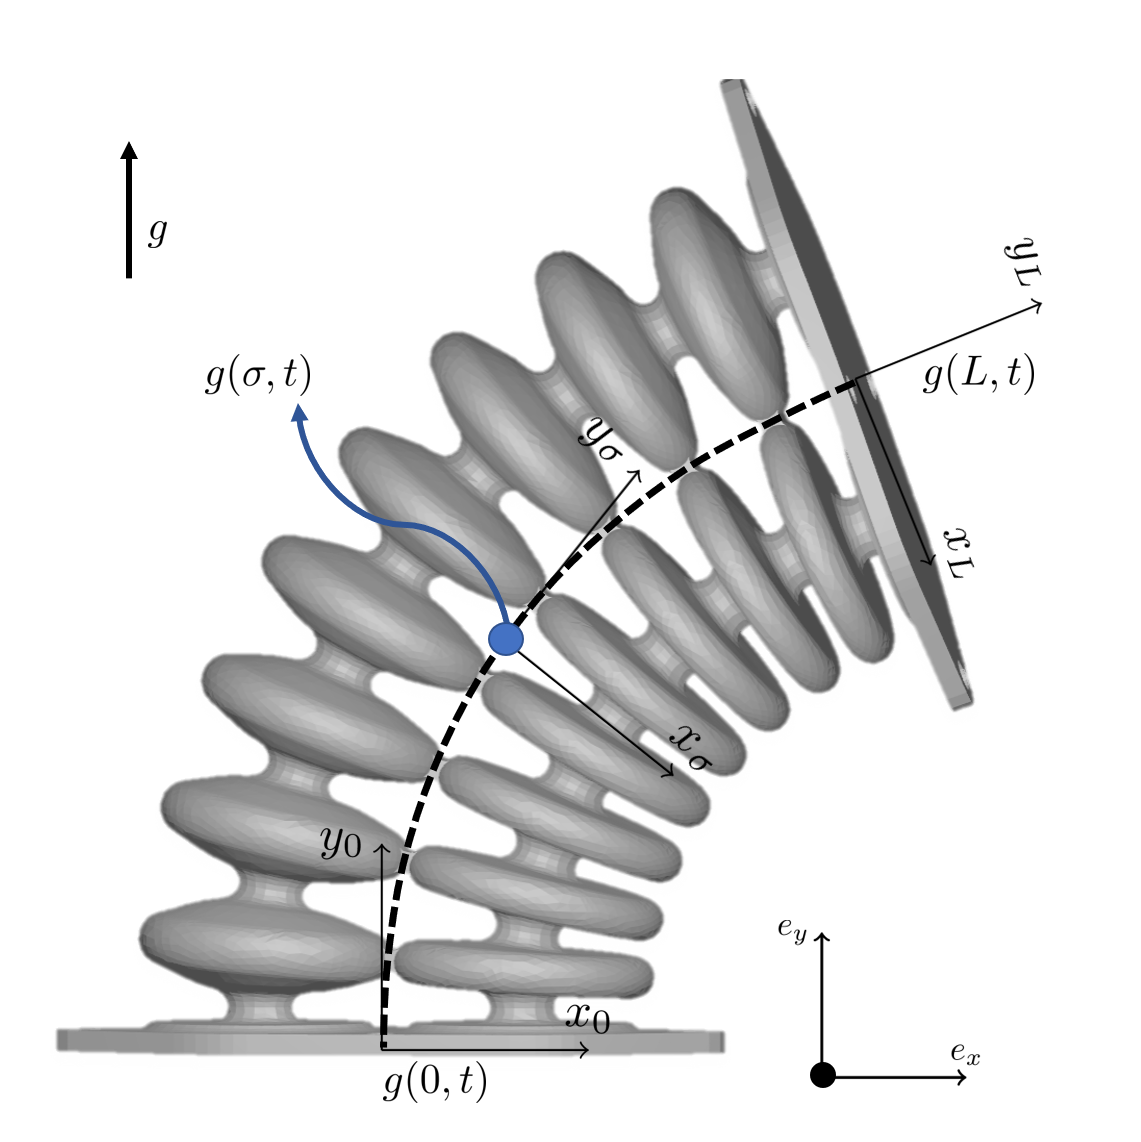
\includegraphics[width=\textwidth]{Figures/Chapter2/actuatorschematic.png}
    \vspace{15pt}
    \caption{Soft robot manipulator with a two-dimensional backbone curve $g(\sigma,t)$.}
    \label{fig2:kinematicschematic}
\end{minipage}
\end{figure}





\section{Cosserat beam theory applied to soft robot manipulator}

To describe the kinematics of the soft robot, a Cosserat beam model is employed \cite{Boyer2019}. This beam model can be thought of as a continuous one-dimensional curve representing the robot's backbone. This backbone is represented in Figure \ref{fig2:kinematicschematic} as the dashed black curve. This curve describes the configuration of the soft robot as a function of space and time. Therefore, this function is dependent on spatial coordinate $\sigma \in \mathbb{X}$ within bounded spatial domain $\mathbb{X} \in [0,L] \subset \mathbb{R}$, where $L$ is the relaxed manipulator length. Furthermore, a temporal coordinate $t \in \mathbb{T}$ with $\mathbb{T} \subset [0,T]$ is defined, where $T$ is the finite time horizon within the time domain. Since the robot's task-space is a two-dimensional plane, the rotation of any point $\sigma$ at time instance $t$ can given by rotation matrix $R(\sigma,t) \in \mathbb{SO}(2)$. The matrices in $\mathbb{SO}(2)$ represent the special orthogonal group within Lie group theory. This matrix expresses rotation of points on a two-dimensional surface relative to the origin. Similarly, the position of that point is given by position vector $s(\sigma,t) \in \mathbb{R}^2$. Therefore, the Cosserat beam model creates a local frame at $\sigma$ tangential to curve $g(\sigma,t)$. This allows to describe position and rotation for any point $\sigma$ and time instance $t$ along the backbone of the soft manipulator by \cite{Caasenbrood2020},


\begin{equation}
    g(\sigma,t) := \begin{bmatrix}  R(\sigma,t) & s(\sigma,t) \\ 0_2^\top & 1 \end{bmatrix} \in \mathbb{SE}(2),
    \label{eq2:g}
\end{equation}

where $\mathbb{SE}(2)$ represents the group of special euclidean matrices that represent rigid-body transformations on $\mathbb{R}^2$, namely rotations and translations \cite{Sola2018}. The strain field and velocity field of the manipulator exist in the tangent space of $\mathbb{SE}(2)$, and thereby an element of $\mathfrak{se}(2)$, i.e. the Lie algebra of $\mathbb{SE}(2)$. To derive forward kinematics, another assumption has to be made for this backbone curve $g(\sigma,t)$.

\begin{theorem}
Curve  $g(\sigma,t)$ is a continuously differentiable function on $\mathbb{T}$ and on $\mathbb{X}$
\end{theorem}

This assumption demands that derivatives of the backbone with respect to time and space are also continuous. These derivatives are essential in determining the strain and velocity field of the soft robot. This strain field allows determining the time-invariant forward kinematics. Whilst the velocity field will be used in determining the system dynamics. First, the forward kinematic problem is solved by computing the strain field.



\section{Computation of the manipulator's strain field}

The strain field allows studying strains along the backbone curve. To find the strain the backbone curve is differentiated with respect to the spatial domain. Throughout this work derivatives with respect to the spatial domain are indicated by a `prime', likewise time derivatives are indicated by a `dot'. The local strain can be found by differentiating (\ref{eq2:g}) with respect to space. This results in the following partial differential equation (PDE) \cite{Caasenbrood2020}, 

\begin{equation}
   g' = \frac{\partial g}{\partial \sigma} = g \hat{\xi} \hspace{10pt} \implies \hspace{10pt}  \hat{\xi}(\sigma,t) := g^{-1}g' = \begin{bmatrix} 0 & -\kappa & \epsilon_x  \\ \kappa & 0 & \epsilon_y \\ 0 & 0 & 0 \end{bmatrix} \in  \mathfrak{se}(2),
    \label{eq2:dgdsigma}
\end{equation}

where $\hat{\xi}(\sigma,t)$ is the space-twist field. Since the problem restricts itself to a single plane there is only one rotation. This rotation is described by curvature strain $\kappa$. This curvature is expressed by a $2 \times 2$ skew-symmetric matrix obtained by $\frac{d}{d\sigma}R(\sigma,t)R^\top(\sigma,t) \in \mathfrak{so}(2)$, where $\mathfrak{so}(2)$ is the Lie algebra of the Lie group $\mathfrak{SO}(2)$. Furthermore, $\epsilon_x$ and $\epsilon_y$ express the stretch-shear strain in perpendicular and tangential, respectively. These skew-symmetric curvature strain and stretch-shear strain combined are within the Lie group $\mathfrak{se}(2)$ \cite{Sola2018}. It shall be clear that for the studied soft robot, shear $e_x$ can not be actively controlled. The matrix $\hat{\xi}(\sigma,t)$ effectively only contains three unique non-zero elements. Therefore, isomorphism of the Lie group $\mathfrak{se}(2)$ allows $\hat{\xi}(\sigma,t) \longmapsto \xi(\sigma,t)$. This allows to equivalently express these curvature strain and stretch-shear strain in a column vector as $\xi(\sigma,t):= [\kappa(\sigma,t) \hspace{3pt} \epsilon_x(\sigma,t) \hspace{3pt} \epsilon_y(\sigma,t) ]^\top \in \mathbb{R}^3 \cong \mathfrak{se}(2)$.

The PDE of (\ref{eq2:dgdsigma}) describes the forward kinematics, which is essential for computing the robot's configuration. It is useful to transform this PDE to an ordinary differential equation (ODE), as this allows for faster computation and controller design. This transformation reduces the original infinite degree of freedom system to a predefined dimension. To be able to transform the system, the following assumption is made: 

\begin{theorem}

$\forall t \in \mathbb{T}$ and $\forall \sigma \in \mathbb{X}$, strain $\xi_i(\sigma,t)$ can be written as an infinite expansion of the form \cite{Caasenbrood2020},

\begin{equation}
\xi_i(\sigma,t) = \sum_{k=1}^\infty \varphi_k(\sigma)q_{i,k}(t) + \xi_{i,0}(\sigma), \hspace{20pt} \forall \sigma \in \mathbb{X}, \forall t \in \mathbb{T} \hspace{2pt} \text{and} \hspace{2pt} i \in \{1,2,3\},
\label{eq2:strainexact}
\end{equation}

in which $\xi_{i}$ is the $i^{\text{th}}$ entry in the curvature-strain vector $\xi(\sigma,t)$. Furthermore, $k \in \mathbb{N}^+$ is the index of the summation consisting of positive integers. The initial strain of the undeformed soft robot is given by $\xi_{i,0}$, and $\varphi_k(\sigma)$ is a set of basis shape functions evaluated at spatial instance $\sigma$, and $q_{i,k}(t)$ a column vector with modal coefficients. 
\end{theorem}

To be precise on this notation, each strain in column vector $\xi(\sigma,t)$ is described by an infinite summation. A single strain is denoted by $\xi_i(\sigma,t)$, with $i$ being the index of that strain. Column vector $q(t)$ contains modal coordinates for all strains in $\xi(\sigma,t)$ for each index $k$. Entry $\xi_{i,0}$ expresses the initial strain present in the undeformed system. Hence, $\hat{\xi}_0(\sigma,t) \in \mathfrak{se}(2) \cong \mathbb{R}^3$. 

This assumption allows transforming the PDE of (\ref{eq2:dgdsigma}) to an ODE by exploiting the Galerkin reduction method \cite{Galerkin}. This method projects the infinite-dimensional system onto a subspace of finite dimension containing basis elements of the expected solution. Each strain is approximated by a finite number of shape functions. Every shape function has a certain contribution to the complete solution. Increasing the number of the shape functions allows studying more complex configurations. The reduction of the system's dimension implies that higher-order dynamics are not captured and thus robustness should be taken into account. To transform the PDE in (\ref{eq2:dgdsigma}), the components of the strain field $\xi(\sigma,t)$ are approximated using a finite number of shape functions as,

\begin{equation}
    [\xi_i(\sigma,t)]_N = \sum_{k=1}^N \varphi_k(\sigma)q_{i,k}(t) + \xi_{i,0}(\sigma) \hspace{15pt} \text{with} \hspace{15pt} \forall \sigma \in \mathbb{X}, \hspace{2pt} t \in \mathbb{T}  \hspace{4pt} \text{and} \hspace{4pt} i \in \{1,2,3\},
    \label{eq2:strainapprox}
\end{equation}

where $N \in \mathbb{N}^+$ is the number of truncations used to approximate strain $\xi_i(\sigma,t)$. Vector $q(t) \in \mathbb{R}^{3 \times N}$ only contains time-dependent modal coordinates. These modal coordinates can be viewed as coefficients expressing the contribution of individual mode shapes to the entire strain approximation. The modal coordinates used here are analogous to for example joint angles as used in traditional robotics. Furthermore, it should be clear that the initial internal deformation $\xi_{i,0}(\sigma)$ is time-invariant. For the studied soft robot the initial deformation is given as $\xi_0 = [0 \hspace{3pt} 0 \hspace{3pt} 1]^\top$. This means that the undeformed robot is either in an upright or down configuration, i.e. no curvature $\kappa_0 = 0$. Furthermore, the strain in horizontal direction $\epsilon_{x,0} = 0$. The stretch in vertical direction $\epsilon_{y,0} = 1$, which corresponds to the soft robots undeformed length $L$. The square brackets around $[\xi(\sigma,t)]_N$ indicate it is an approximation with truncation $N$. 

There exist multiple variants of shape function polynomials that can be used in approximating strain. In this work, Legendre polynomials are considered which are given by,

\begin{equation}
    \varphi_{k} = \frac{1}{2^{k-1} k-1!} \frac{d^{k-1}}{d\sigma^{k-1}}\Big(\Big(\frac{2\sigma}{L}-1\Big)^2-1\Big)^{k-1},
    \label{eq2:shapefunction}
\end{equation}

where $\varphi_k$ represents a particular (strain) shape present in the soft robot on the bounded domain $[0,L]$. It is important to understand that the set of basis function $\{\phi_k\}_{k=1}^N$ has an order (which is intrinsically the case for Legendre polynomials) such that the first shape function $\varphi_1$ contributes most to the reconstruction of strain field $\xi(\sigma,t)$. Increasing the number of shapes yields a better description of the actual strain present in the manipulator. However this is at the cost of computational speed. As an illustrative example, the first four shape functions have been evaluated on the domain $[0,1]$ and are displayed in Figure \ref{fig2:shapefunction}.

\begin{figure}[H]
    \centering
    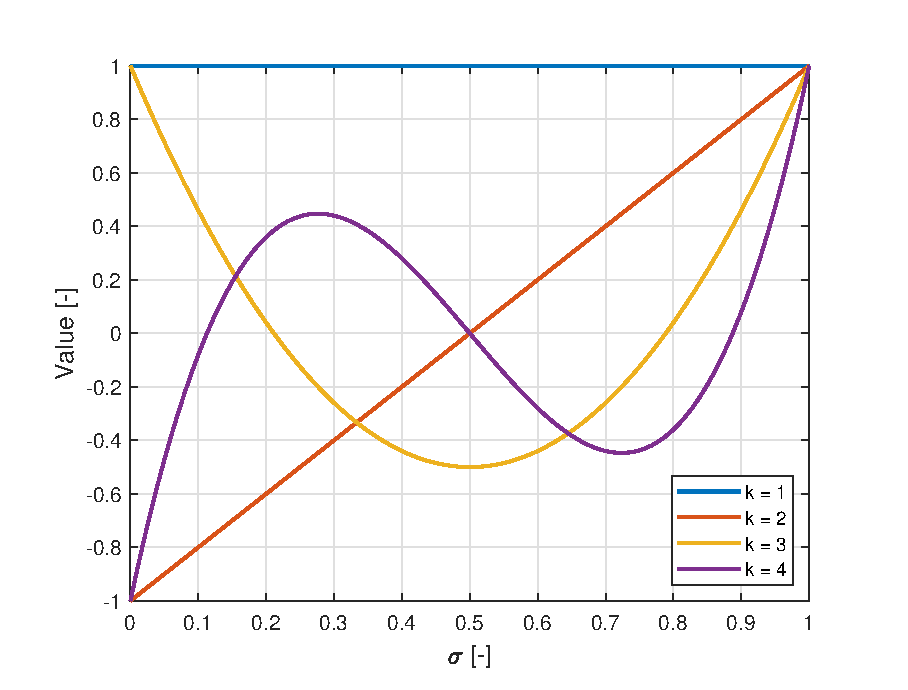
\includegraphics[width = 0.7\textwidth ]{Figures/Chapter2/shapefunction.eps}
    \caption{First 4 Legendre shape functions on domain $[0 \hspace{4pt} 1]$.}
    \label{fig2:shapefunction}
\end{figure}

Figure \ref{fig2:shapefunction} shows that for $k=1$ the resulting Legendre polynomial is equal to $1 \hspace{2pt} \forall \sigma$. Furthermore, the figure shows that each degree of shape-function takes more complex shapes. Therefore increasing the order of shape functions allows the model to describe more complex robot configurations. To avoid coupling between the states, these shape functions must be orthogonal to each other. This means that $\int_\mathbb{X} \varphi_i \varphi_j d \sigma = 0$ for any $i \neq j$ and non-zero otherwise. The strain approximation of (\ref{eq2:strainapprox}) can be written as a $N$-th order expansion as,



\begin{equation}
\begin{aligned}
    \begin{bmatrix}\xi(\sigma,t)\end{bmatrix}_N = & \hspace{5pt}  (B_a \otimes [ \varphi_1(\sigma) \dots \varphi_N(\sigma) ])q(t) + \xi_0 \\ = &  \underbrace{ \begin{bmatrix}
    \varphi_1(\sigma) & \dots  & \varphi_N(\sigma) & \dots     & 0      & \dots  &  0 \\
    \vdots    & \ddots & \vdots    & \ddots    & \vdots & \ddots & \vdots \\
    0         & \dots  & 0         & \dots     & \varphi_1(\sigma) & \dots & \varphi_N (\sigma)
    \end{bmatrix}}_{\Phi(\sigma)} \begin{bmatrix} q_{1,1}(t) \\ \vdots \\ q_{3,N}(t) \end{bmatrix} +  \begin{bmatrix} \xi_{1,0} \\ \vdots \\ \xi_{3,0}   \end{bmatrix}
    \end{aligned},
\label{eq2:xishape}
\end{equation}

where $\Phi(\sigma) \in \mathbb{R}^{3 \times mN}$ is the Kronecker-product between matrix $B_a \subseteq \text{span} \hspace{2pt} I_3$ and transposed vector $\varphi(\sigma) \in \mathbb{R}^N$. Integer $m$ is defined as the number of active strains in the system. In this context, the active strains are strains that can be actively controlled. For the considered soft robot, this is the curvature $\kappa$ and the vertical elongation $\epsilon_y$. Hence, $m=2$ for this system. Based on these active strains, selection matrix of unconstrained strains can be defined as,

\begin{equation}
    B_a = \begin{bmatrix}
    1 & 0 \\
    0 & 0  \\
    0 & 1  \\
    \end{bmatrix}.
    \label{eq2:Ba}
\end{equation}

The entries of selection matrix $B_a$ tells that only the first and third strain are free. This implies that only these two strains are approximated. Now the reduction method is detailed, another assumption is made regarding the maximum truncation $N$ in the strain approximation.

\begin{theorem}
The strains induced by actuating the soft robot under basic operating conditions can be captured by truncation of $N = 1$. 
\end{theorem}

Based on this assumption, and the shape function polynomials of (\ref{eq2:shapefunction}) a first order approximation of the strains is made. Substitution of the provided expressions for $B_a$ (\ref{eq2:Ba}) and $\xi_0$ into (\ref{eq2:xishape}) the strains of the soft robot can be described by,


\begin{equation}
    \begin{bmatrix}\xi(t)\end{bmatrix}_1 =\underbrace{B_a \otimes [\varphi_1]}_{\Phi(\sigma)} q(t) + \xi_0  =  \underbrace{\begin{bmatrix}
    1 & 0  \\
    0 & 0  \\
    0 & 1
    \end{bmatrix}}_{\Phi} \begin{bmatrix} q_{1,1}(t) \\  q_{2,1}(t) \end{bmatrix} +  \begin{bmatrix} 0 \\ 0 \\ 1   \end{bmatrix},
\label{eq2:xiapprox}
\end{equation}

where it can be concluded that the approximated strain becomes space-invariant. Given that for a first-order truncation the shape function is equal to $1 \hspace{2pt} \forall \sigma$, as is shown in Figure \ref{eq2:shapefunction}. Therefore, the Kronecker product between $B_a$ and $[\varphi_1]$ results in a space-invariant matrix $\Phi$ which has the same entries and structure as $B_a$. Furthermore, it can be seen that the second component of strain vector $[\xi(\sigma,t)]_1$, corresponding to elongation $\epsilon_x = 0 \hspace{3pt} \forall \hspace{3pt} \sigma $ and $ \forall \hspace{3pt} t$. This allows us to define the modal coordinate vector as,


\begin{equation}
q(t) = \begin{bmatrix} q_{1,1}(t) \\ q_{2,1}(t) \end{bmatrix} = \begin{bmatrix} \kappa(t) \\ \epsilon_y(t) \end{bmatrix} = \begin{bmatrix} \kappa(t) \\ \epsilon(t) \end{bmatrix}.
\end{equation}

Since $\epsilon_x = 0$, a new notation for the strains is proposed. Throughout this work, we will use ``elongation" or $\epsilon$ to address strain $\epsilon_y$. Likewise, ``curvature'', ``rotation'' or  $\kappa$ are used interchangeably to refer to curvature $\kappa$. Approximating strains and curvatures with a single shape function will essentially reduce this Cosserat model to the piece-wise constant curvature (PCC) model as discussed in Chapter \ref{chapter1}. From (\ref{eq2:shapefunction}) it can be concluded that all shape functions yield 1 for $k=1$. In that specific case, the modal coordinates $q(t)$ will be equal to $\kappa(t)$ and $\epsilon(t)$, respectively. From this point onward, only a single shape function is used to approximate the strains and curvatures of the robot. 

In the next section, the forward kinematic problem is solved with the described strain approximation.




\section{Forward kinematics of the manipulator}

The forward kinematic problem of (\ref{eq2:dgdsigma}) for the
planar soft robot is solved by spatial integration over domain $[0,L]$. At each discrete increment the strain field $[\xi(t)]_1$ is approximated by (\ref{eq2:xiapprox}). A standard ODE solver such as $\verb+ode45.m+$ in \MATLAB \cite{MATLAB2020} will suffice. The chosen initial condition is $g(0,t) = I_3 \hspace{2pt} \forall t$, which corresponds to zero rotation and zero strain at $\sigma = 0$. Furthermore, the modal coordinates are chosen constant as $q = q(t) \hspace{2pt} \forall t$. 

Figure \ref{fig1:forward_kinematic} shows the result of the solved forward kinematic problem. The initial position is obtained for zero curvature and elongation. It can be seen that the undeformed length of the soft robot $L$ is equal to 64.5 mm. To obtain the deformed modal coordinate $q$ was chosen equal to $[-17,0.1]^\top$. Physically this implies a clockwise rotation and a 10\% elongation of the soft robot.


\begin{figure}[H]
    \centering
    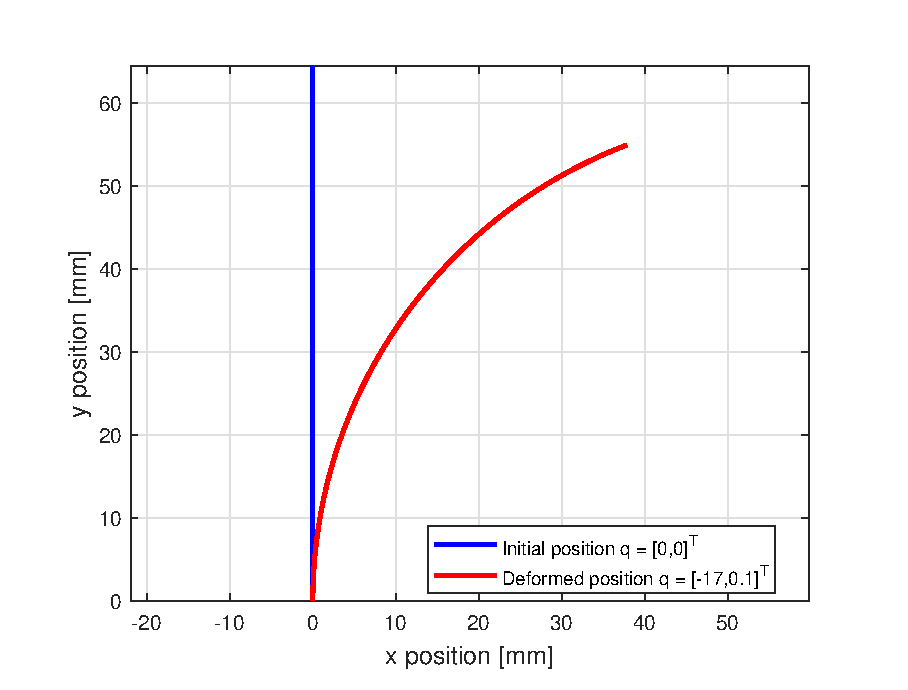
\includegraphics[width = 0.65\textwidth]{Figures/Chapter2/fkin1701.eps}
    \caption{Initial configuration and deformed configuration solving the forward kinematic model for $q = [-14,0.1]^\top$.}
    \label{fig1:forward_kinematic}
\end{figure}



Besides a forward kinematic model, a numerical inverse kinematic solver was programmed. This allows defining a position in planar Cartesian coordinates and retrieve the modal coordinates belonging to that position. The algorithm will minimize the distance between the desired end-effector position and reachable end-effector position given the number of truncations $N$. It shows the model's flexibility when using multiple shape functions. The algorithm is further detailed in Appendix \ref{app:chap2}. 

For now, the time dependency of modal coordinate vector $q(t)$ has been neglected. However, to determine the dynamics of the system it is crucial to consider the time-variance of the system. To do so, the velocity kinematics of the system are derived in the next section.


\section{Velocity kinematics of the manipulator}

The velocity kinematics allows studying velocities along the backbone curve. Similar to the spatial derivative, backbone curve $g(\sigma,t)$ can be differentiated with respect to time. This differentiation results in \cite{Caasenbrood2020}, 

\begin{equation}
  \Dot{g} = \frac{\partial g}{\partial t} = g \hat{\eta} \hspace{10pt} \implies \hspace{10pt}  \hat{\eta}(\sigma,t) := g^{-1}\dot{g} = \begin{bmatrix} 0 & -\omega & v_x \\ \omega & 0 & v_y \\
  0& 0 & 0 \end{bmatrix} \in  \mathfrak{se}(2)
    \label{eq2:dgdt}
\end{equation}

which describes the time-twist field of a local frame at $\sigma$ at time $t$. Since a planar case is considered, there is a single angular velocity. This angular velocity is expressed by a $2 \times 2$ skew-symmetric matrix obtained by $\frac{d}{dt}R(\sigma,t)R^\top(\sigma,t) \in \mathfrak{so}(2)$. The linear velocities in perpendicular and tangential direction are described by $v_x$ and $v_y$, respectively. Therefore, $\hat{\eta} \in \mathfrak{se}(2)$ effectively contains angular and linear velocities among the backbone curve. Due to the isomorphism of $\mathfrak{se}(2) \longmapsto \mathbb{R}^3$, all velocities can equivalently be stored in column vector $\eta(\sigma,t) := [\omega(\sigma,t) \hspace{3pt} v_x(\sigma,t) \hspace{3pt} v_y(\sigma,t)]^\top \in \mathbb{R}^3 \cong \mathfrak{se}(2)$ \cite{Sola2018}.


Using the equality of mixed partial derivatives, at each instant of space and time $\frac{\partial}{\partial t}g' = \frac{\partial}{\partial \sigma}\dot{g}$ holds \cite{Caasenbrood2020}. Employing general rules of substitution and actions in Lie space it can be proven that the spatial derivative of the velocity field can be written as  \textcolor{blue}{\cite{Caasenbrood2020}}, \cite{Boyer2019},

\begin{equation}
    \eta'(\sigma,t)= (\text{Ad}_{g(\sigma,t)^{-1}})'\text{Ad}_{g(\sigma,t)} \eta(\sigma,t) + \Dot{\xi}(\sigma,t) \hspace{10pt} \text{with} \hspace{10pt} \text{Ad}_{g(\sigma,t)} = \begin{bmatrix} 0_2^\top & 1 \\ \Tilde{s}(\sigma,t) & R(\sigma,t)  \end{bmatrix} \in \mathbb{R}^{3\times 3}
    \label{eq2:etadif}
\end{equation}


where $\text{Ad}_g \in \mathbb{R}^{3 \times 3}$ \cite{2DLie} is the adjoint mapping of $g(\sigma,t)$ \cite{Sola2018}. Vector $\Tilde{s}$ is defined as $[s_2(\sigma,t) \hspace{5pt} -s_1(\sigma,t)]^\top$ \cite{2DLie}, which can be derived from the adjoint action defined for the Lie group $\mathbb{SE}(3)$. This adjoint mapping allows velocities expressed in local frame $g(\sigma,t)$ to be mapped to frame $g(0,t)$, which coincides with the Cartesian coordinate frame. The complete derivation of (\ref{eq2:etadif}) is presented in Appendix \ref{app:chap2}. 

An analytic solution to (\ref{eq2:etadif}) can be found by integrating the equation over spatial domain $[0,\sigma]$. It is given that the soft robot is fixed at one end. Therefore the boundary conditions $\eta_0 = 0_{3}^\top$ and $g_0 = I_{3}$ can be imposed. This physically means that for $\sigma = 0$ velocity, strain and curvature are equal to zero. Integrating over domain $[0,\sigma]$ will give accordingly  \cite{Caasenbrood2020},

\begin{equation}
  \begin{bmatrix} \eta(\sigma,t)\end{bmatrix}_1 = \text{Ad}_{[g(\sigma,t)]_1^{-1}} \int_0^{\sigma} \text{Ad}_{[g(\sigma,t)]_1} \Phi \hspace{2pt} d \sigma  \hspace{2pt} \dot{q}(t) = [J(\sigma,t)]_1\dot{q}(t),
    \label{eq2:J}
\end{equation}

here an expression for the geometric Jacobian $[J(\sigma,t)]_1 \in \mathbb{R}^{3\times 2}$ is obtained \cite{Caasenbrood2020}, for a first-order strain truncation. This Jacobian maps modal coordinate velocity to linear and angular velocities in Cartesian coordinates along the backbone curve. Recall that two active degrees of freedom are considered, that are strain $\epsilon$ in the y-direction and curvature strain $\kappa$. Therefore, the modal coordinate vector $q(t)$ is of dimension two. The geometric Jacobian maps the modal coordinate velocity $\dot{q}(t)$ to velocities in the Euclidean space. The velocity of a point with respect to a reference in 2-dimensional Euclidean space is described by 3 components. From the fixed reference point at $g(0,t)$, these velocities are one angular velocity, and two linear velocities in horizontal en vertical direction, respectively. This complies with the dimension of the Jacobian matrix. As can be seen, this Jacobian matrix is space-variant. Besides relating modal coordinate velocity to Cartesian velocity, the Jacobian can be used on position level as,

\begin{equation}
    r(\sigma,t) = [J(\sigma,t))]_1q(t),
\end{equation}

which implies that modal coordinates $q(t)$ can also be mapped to a position vector $r\in \mathbb{R}^3$ in Euclidean space. This position vector contains rotation, horizontal and vertical position as $[\theta \hspace{3pt} x \hspace{3pt} y]^\top$, respectively. Therefore this Jacobian is of valuable use for further system analysis. It can for instance be used in path-planning, as the Jacobian inverse can map Cartesian coordinates to modal coordinates. Furthermore, it can be used in controller design. However, in the next section, the Jacobian will be used for deriving the dynamics of the soft robot. 


\section{Dynamic model derivation of the manipulator}

To study the dynamic behaviour of the soft robot, a dynamic model is derived. In this model the manipulator's dynamics and air pump dynamics are regarded as a set of coupled equations. The manipulator dynamics are captured by non-linear function $f(x_1)$, which is dependent on state vector $x_1 = [ q \hspace{4pt} \dot{q} ]^\top \in \mathbb{R}^4$. The linear input function $g(x_1,x_2)$ is dependent on state variables $x_1$ and $x_2$, where the latter is defined as $x_2 = [p_1 \hspace{4pt} p_2]^\top \in \mathbb{R}^2$. The air pumps dynamics are captured by a linear state-space model. In this model, linear system matrix $A \in \mathbb{R}^{2\times 2}$ captures the pump dynamics. The pressure is regulated with input vector $V(t) \in \mathbb{R}^2$ describing the Volt input supplied to each individual air pump. The effects of the input $V(t)$ on the pressure is captured by control input matrix $B \in \mathbb{R}^{2\times2}$. Hence, the system of coupled equations can be formulated as,




\begin{equation}
    \dot{x}_1  = f(x_1) + g(x_2), 
       \label{eq2:nonlineq1}
    \end{equation}
    \begin{equation}
    \dot{x}_2 = Ax_2 + BV(t). 
    \label{eq2:nonlineq2}
\end{equation}

First, the soft robot dynamics as described in (\ref{eq2:nonlineq1}) are derived. Then, the air pump dynamics of (\ref{eq2:nonlineq2}) are provided. Eventually, the two equations are merged to a single non-linear state-space representation capturing the overall system dynamics. To model the soft robot dynamics the following assumption is made:

\begin{theorem}
The soft robot's dynamics can be modelled as a non-linear mass-spring-damper system, assuming that the system is not affected by Coriolis effects. Gravitational effects are deemed insignificant due to the low system mass.
\end{theorem}

Neglecting the influence of gravity is deemed valid, as the mass of the system is low ($m << 0.1 kg$). Given the system's low mass, and slow operating velocity, the contribution of the Coriolis terms are deemed negligibly small. Therefore, the dynamic model will take the following structure,


\begin{equation}
    M(q)\Ddot{q} + D\dot{q} + K(q)q = \nu(p),
    \label{eq2:simp_model}
\end{equation}


where $M(q)$ is the non-linear mass matrix. Since the Jacobian matrix is space-variant, it is assumed that the mass matrix will be space-variant too. This makes the system non-linear. Furthermore, $D$ is a damping matrix with assumed linear damping properties. Matrix $K(q)$ captures the non-linear stiffness. It is known that the elastomer of which the soft robot is composed deforms non-linearly. The input of the system is $\nu(p) \in \mathbb{R}^2$. This input vector consists of a moment and force acting on the system which is a function of pressure. 

The dynamic model as posed in (\ref{eq2:simp_model}) can be obtained based on the Lagrangian method. The Lagrangian is defined as $\mathcal{L} = \mathcal{T} -\mathcal{V}$ which expresses the energy difference between kinetic energy $\mathcal{T}$ and potential energy $\mathcal{V}$. Exact expressions for the kinetic energy and potential energy of the system are given by, respectively {\cite{Caasenbrood2020},

\begin{equation}
    \mathcal{T} = \frac{1}{2}\int_0^{\sigma} \eta(\sigma,t)^\top \mathcal{M} \eta(\sigma,t) \hspace{2pt} ds \hspace{20pt} \text{and} \hspace{20pt}  \mathcal{V} = \frac{1}{2}\int_0^{\sigma} \xi(\sigma,t)^\top \mathcal{K} \xi(\sigma,t)  \hspace{2pt} ds,
    \label{eq2:T}
\end{equation}


where $\mathcal{M} \in \mathbb{R}^{3\times3}$ and $\mathcal{K} \in \mathbb{R}^{3\times3}$ are a diagonal mass tensor and stiffness tensor, respectively. The approximations for velocity (\ref{eq2:J}) and strain (\ref{eq2:xishape}) can be substituted in this equation to formulate the kinetic and potential energy as follows,

\begin{equation}
    \mathcal{T} = \frac{1}{2}\int_0^{\sigma} \Big([J(\sigma,t)]_1\dot{q}\Big)^\top \mathcal{M} \Big([J(\sigma,t)]_1\dot{q}\Big) \hspace{2pt} ds
\end{equation}

\begin{equation}
\begin{split}
    \mathcal{V} &= \mathcal{V}(q) + \mathcal{V}_0  \\
                &=  \frac{1}{2}\int_0^{\sigma} \big(\Phi q\big)^\top \mathcal{K} \big(\Phi q\big) \hspace{2pt} ds +\frac{1}{2} \int_0^\sigma \xi_0^\top \mathcal{K} \xi_0  \hspace{2pt} ds .
\end{split}
\end{equation}

Above expression allows deriving the Lagrangian equations of motion as \cite{NWouw},

\begin{equation}
    \frac{\partial}{\partial t}\Big( \frac{\partial}{\partial\dot{q}}\mathcal{T}\Big)- \frac{\partial}{\partial q}\mathcal{T} + \frac{\partial}{\partial q}\mathcal{V} = \mathcal{Q}^{nc} \hspace{10pt} \text{with} \hspace{10pt} \mathcal{Q}^{nc} =  \nu(p) - \int_0^\sigma \Phi^\top \mathcal{D} \Phi \dot{q} \hspace{2pt} d \sigma
    \label{eq2:lagrange}
\end{equation}

where $\mathcal{Q}^{nc} \in \mathbb{R}^2$ is a vector containing non-conservative forces acting on the system. One of these non-conservative forces are actuation forces. These actuation forces are captured in vector $\nu(p) \in \mathbb{R}^2$. Another non-conservative force are the damping forces as a result of the energy dissipation in the elastomer. These damping terms are captured in diagonal damping tensor $\mathcal{D} \in \mathbb{R}^{3 \times 3}$. Also note that the approximated strain rate is substituted which, without further prove, can be easily obtained from (\ref{eq2:xiapprox}). Further simplification of (\ref{eq2:lagrange}) and rearranging terms gives,

\begin{equation}
    \int_0^\sigma \Big( \underbrace{[J(\sigma,t)]_1^\top \mathcal{M} [J(\sigma,t)]_1}_{M(q)} \ddot{q} +  \underbrace{\Phi^\top \mathcal{D} \Phi }_{D} \dot{q}    +   \underbrace{\Phi^\top \mathcal{K} \Phi}_{K(q)} q\Big) \hspace{2pt} d\sigma = \nu(p),
\end{equation}

where it becomes clear that $M(q)$, $D(q)$ and $K(q)$ all exist in $\in \mathbb{R}^{2\times2}$, since $[J(\sigma,t)]_1 \land \Phi \in \mathbb{R}^{3 \times 2}$. Since the Coriolis effects are deemed small, the term $\frac{\partial}{\partial q}\mathcal{T} \approx O_2 $ is omitted. Now the expressions for the mass, damping and stiffness matrices are defined, the entries of their tensors are elucidated, respectively.

In the modelling approach, the soft robot kinematics have been described by a one-dimensional backbone curve. To derive the mass matrix, mass properties need to be assigned to this curve. Therefore, the backbone curve is discretized and an infinitely thin slice of the cross-section of the soft robot is considered. To derive the mass tensor of the system the following assumption is made.

\begin{theorem}
The inertial properties of the soft robot can be determined by considering an infinitely thin slice ($d \sigma \xrightarrow[]{}0$) in the transverse direction and regarding it as a solid cuboid, which is independent of the state $q$ or $\sigma$.
\end{theorem}

Figure (\ref{fig:massapprox}) shows such a discretized cross section. In this figure the blue marked area reflects a solid cuboid with height $h$, width $w$, density $\rho$ and slice thickness $d\sigma$. 


\begin{figure}[H]
    \centering
    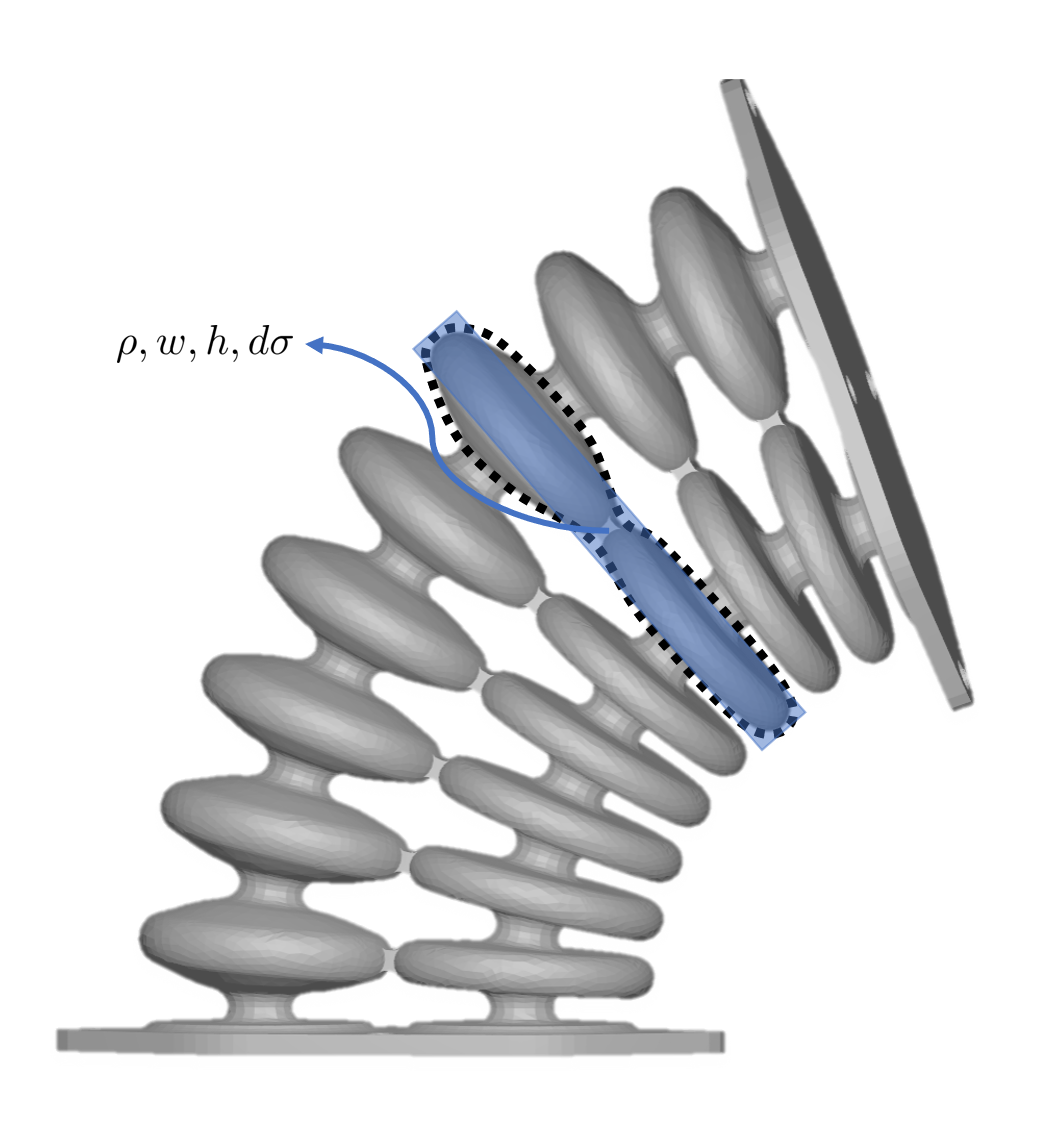
\includegraphics[width = 0.4\textwidth]{Figures/Chapter2/massapprox.png}
    \caption{Inertial properties can be determined by regarding an infinitely thin slice. The cross section is then viewed a solid cuboid.}
    \label{fig:massapprox}
\end{figure}


The mass tensor $\mathcal{M}$ then takes the following form,

\begin{equation}
    \mathcal{M} = \begin{bmatrix} \frac{1}{12}\rho w^2 & 0 & 0 \\
                                   0 & \rho & 0 \\
                                   0 & 0 & \rho \end{bmatrix}\hspace{5pt} \text{with} \hspace{5pt} \rho = \frac{m}{L}
\end{equation} 




where $m$ is the total mass of the robot. The first entry expresses mass moments of inertia, related to the curvature acceleration of the soft robot. The last two entries relate to the linear acceleration of the centre of mass of the cuboid. Based on equation (\ref{eq2:T}) the space-time variant mass matrix can be expressed as  \cite{Caasenbrood2020}, 


\begin{equation}
    M(q)) = \int_0^{\sigma} [J(\sigma,t)]_1^\top \mathcal{M}(\sigma)[J(\sigma,t)]_1  \hspace{2pt}ds,
\end{equation}

where it should be noted this mass-matrix has off-diagonal entries related to the non-linear Jacobian matrix. 

It is assumed that the polymer of which the soft robot is composed has linear damping characteristics. Therefore, the damping matrix is constant and can be described by \cite{Caasenbrood2020},

\begin{equation}
    D = \int_0^\sigma \Phi^\top \mathcal{D} \Phi \hspace{2pt} ds  := \text{diag}([D_\kappa, D_\epsilon]),
\end{equation}

which has no off-diagonal terms. This means that there are two damping parameters $D_\kappa$ and $D_\epsilon$, which are related to curvature velocity and strain rate, respectively. These damping parameters will be chosen iteratively, as it is impossible to measure damping properties experimentally. The system can not be actuated such that a single degree of freedom is excited. 

It is given that the polymer has non-linear stiffness properties, which implies that stiffness matrix $K(q)$ is space-variant. The stiffness matrix is described as \cite{Caasenbrood2020},

\begin{equation}
    K(q) = \int_0^\sigma \Phi^\top \mathcal{K}(q) \Phi \hspace{2pt} ds := \text{diag}([K_\kappa(\kappa), K_\epsilon(\epsilon)]),
\end{equation}

which has no off-diagonal terms. This implies that curvature stiffness $K_\kappa(\kappa)$ and elongation stiffness $K_\epsilon(\epsilon)$ need to be determined. The process of obtaining these non-linear stuffiness's is explained in Chapter \ref{chap3}. Furthermore, the geometric properties and material properties are presented that are necessary to compute the mass tensor. 

The non-linear mass-spring-damper system of (\ref{eq2:simp_model}) can be rewritten to the form as introduced by (\ref{eq2:nonlineq1}). This gives the non-linear state-space expression of the soft robot dynamics as,


\begin{equation}
    \underbrace{\begin{bmatrix}\dot{q}\\ \ddot{q}  \end{bmatrix}}_{\dot{x}_1}   = \underbrace{  \begin{bmatrix} O_{2} & I_{2} \\ -M(q)^{-1}K(q)  & -M(q)^{-1} D \end{bmatrix}   \begin{bmatrix} q \\ \dot{q} \end{bmatrix} }_{f(x_1)}  +      \underbrace{ \begin{bmatrix} O_{2} \\ M(q)^{-1}   \end{bmatrix}       \begin{bmatrix} \nu_1(p) \\ \nu_2(p)  
    \end{bmatrix} }_{g(x_1,x_2)}, 
    \label{eq4:SS}
\end{equation}

where the physical interpretation of $\nu_1(p)$ is a pressure induced moment causing the soft robot to bend. Input $\nu_2(p)$ can be regarded as a pressure causing the soft robot to elongate.



\section{Air pump model}


At this point, the dynamic model of the soft robot has been derived. However, actuation has a major influence on the combined system dynamics. Therefore, it is important to include pressure dynamics as well. Each bellow of the soft robot is pressurized using a diaphragm air pump. These air pumps compress air using membranes. The speed at which the membranes open and close determines the rate at which pressure increases. This speed is regulated by supplying a DC voltage to the electric motor which opens and closes the membranes. To model the air pump dynamics the following assumption is made.

\begin{theorem}
The air pumps used for actuating the soft robot have identical dynamics that can be described by a first-order linear model.
\end{theorem}

This assumption allows to formulate the pump dynamics as,

\begin{equation}
 \underbrace{\dot{p}}_{\dot{x_2}}  = \underbrace{\begin{bmatrix} -\lambda_1 & 0 \\ 0 & -\lambda_1 \end{bmatrix} p}_{Ax_2} + \underbrace{\begin{bmatrix} \lambda_2 & 0 \\ 0 & \lambda_2 \end{bmatrix} V(t)}_{BV(t)},
    \label{eq2:pumpmodel}
\end{equation}

where $p =  [p_1 \hspace{4pt} p_2]^\top$ is the bellow pressure regulated by input Voltage $V(t)$. Constant $\lambda_1 \in \mathbb{R}^+$ represents the system's resistance to a pressure increase and is dependent on actual system pressure. Parameter $\lambda_2 \in \mathbb{R}^+$ is a constant that incorporates the pressure increase relative to the Volt input signal. Additionally, it should be noted that this $\lambda_1$ also acts as some deflation coefficient. For zero volt input, the system pressure decreases with a rate relative to the system pressure. Both of these parameters can be obtained through experimental analysis. Note that in (\ref{eq2:pumpmodel}) the structure of (\ref{eq2:nonlineq2}) can directly be recognized. 







\section{Combined dynamics of the soft robotic system}




The system of equations as presented in (\ref{eq2:simp_model}) and (\ref{eq2:pumpmodel}) can be combined to capture the overall system dynamics. Hereto, control input function $\nu(p)$ needs to be defined. As mentioned, the entries in $\nu(p)$ can be regarded as a moment and force causing the manipulator to bend and elongate, respectively. Therefore, a linear mapping matrix is proposed as $\nu(p) = H p$, where $H \in \mathbb{R}^{2\times 2}$ maps pressure vector $p$ to input moment and force. The overall system dynamics can then be captured by the following state-space representation,

\begin{equation}
     \begin{bmatrix} \dot{x}  \end{bmatrix}   =   \underbrace{ \begin{bmatrix} O_{2\times 2} & I_{2} & O_{2} \\ -M(q)^{-1}K(q)  & -M(q)^{-1} D & O_{2} \\
     O_{2} & O_{2}    & -\lambda_1 I_{2}\ \end{bmatrix}   }_A   \begin{bmatrix} x \end{bmatrix}  + \underbrace{      \begin{bmatrix} O_{2} & O_{2} \\ M(q)^{-1}H & O_{2} \\ O_{2} & \lambda_2 I_{2} \end{bmatrix} }_B      \begin{bmatrix} p_1 \\ p_2  \\ V_1 \\ V_2 \end{bmatrix},
     \label{eq:ssp}
\end{equation}

where matrix $A \in \mathbb{R}^{6\times 6}$ contains the complete system dynamics and matrix $B \in \mathbb{R}^{6\times 4}$ is the control input matrix. State vector $x$ is then defined as $x = [q \hspace{4pt} \dot{q} \hspace{4pt} p]^\top$. Also, note the substitution of $\nu(p) = Hp$, where $H$ can be determined experimentally. 



\section*{Summary}

In this chapter, a dynamic model for the entire system is deduced. Based on the Cosserat beam model a continuous backbone curve is formulated along the centre of the soft robot. This backbone curve is a function of space and time. Differentiating this curve with respect to space allows deriving the forward kinematics. The time derivative of the backbone curve is utilized to derive the Jacobian matrix. This Jacobian matrix allows mapping modal coordinates to Cartesian coordinates. The soft robot dynamics are captured using a non-linear mass-damper-damper model. Based on the Lagrangian method, the mass, damping and stiffness matrices are derived. To model the pump dynamics, a first-order linear model is assumed. The dynamic model of the soft robot is combined with the pump model to create a state-space model. 







%To numerically solve the dynamic model of ,  (\ref{eq2:simp_model}) is reformulated to a second-order state-space formulation as,

%\begin{equation}
%    \underbrace{\begin{bmatrix}\dot{q}\\ \ddot{q}  \end{bmatrix}}_{\dot{x}_1}   = \underbrace{  \begin{bmatrix} O_{2} & I_{2} \\ -M(q)^{-1}K(q)  & -M(q)^{-1} D \end{bmatrix}   \begin{bmatrix} q \\ \dot{q} \end{bmatrix} }_{f(x_1)}  +      \underbrace{ \begin{bmatrix} O_{2} \\ M(q)^{-1}   \end{bmatrix}       \begin{bmatrix} \nu_1(p) \\ \nu_2(p)  
%    \end{bmatrix} }_{g(x_2)}, 
%    \label{eq4:SS}
%\end{equation}

%where the structure of (\ref{eq2:nonlineq1}) can be recognized with state vector $x_1 = [ q \hspace{3pt} \dot{q}   ]^\top =  [\kappa \hspace{3pt} \epsilon \hspace{3pt} \dot{\kappa}  \hspace{3pt} \dot{\epsilon}  ]^{\top}$ and $x_2 = p$. From a physical standpoint, the entries of the input vector $\nu(p)$ can interpreted as a moment and a force acting on the system. The moment $\nu_1$ causes the soft robot to curve, whereas $\nu_2$ can be viewed as a force that induces elongation.
